\chapter{Étude d'un prédicteur de Smith}
Nous allons maintenant passer à l'analyse d'un autre type de correction de systèmes à retard : le prédicteur de Smith. Ce type de correcteur permet d'établir une commande de système retardé en utilisant une estimation du procédé qui sera utilisé en temps $t$ et $t+h$.

\section{Schéma de principe du prédicteur de Smith}
Nous avons dessiné avec \emph{Simulink} le schéma bloc en figure \ref{fig:sch_predicteurSmith}, dans lequel nous avons séparé $\tilde{C}(p)$ (C\_Smith sur le schéma) et  $ G(p) e ^{-hp}$(Procédé dans le schéma).
\begin{figure}[!ht]
\centering
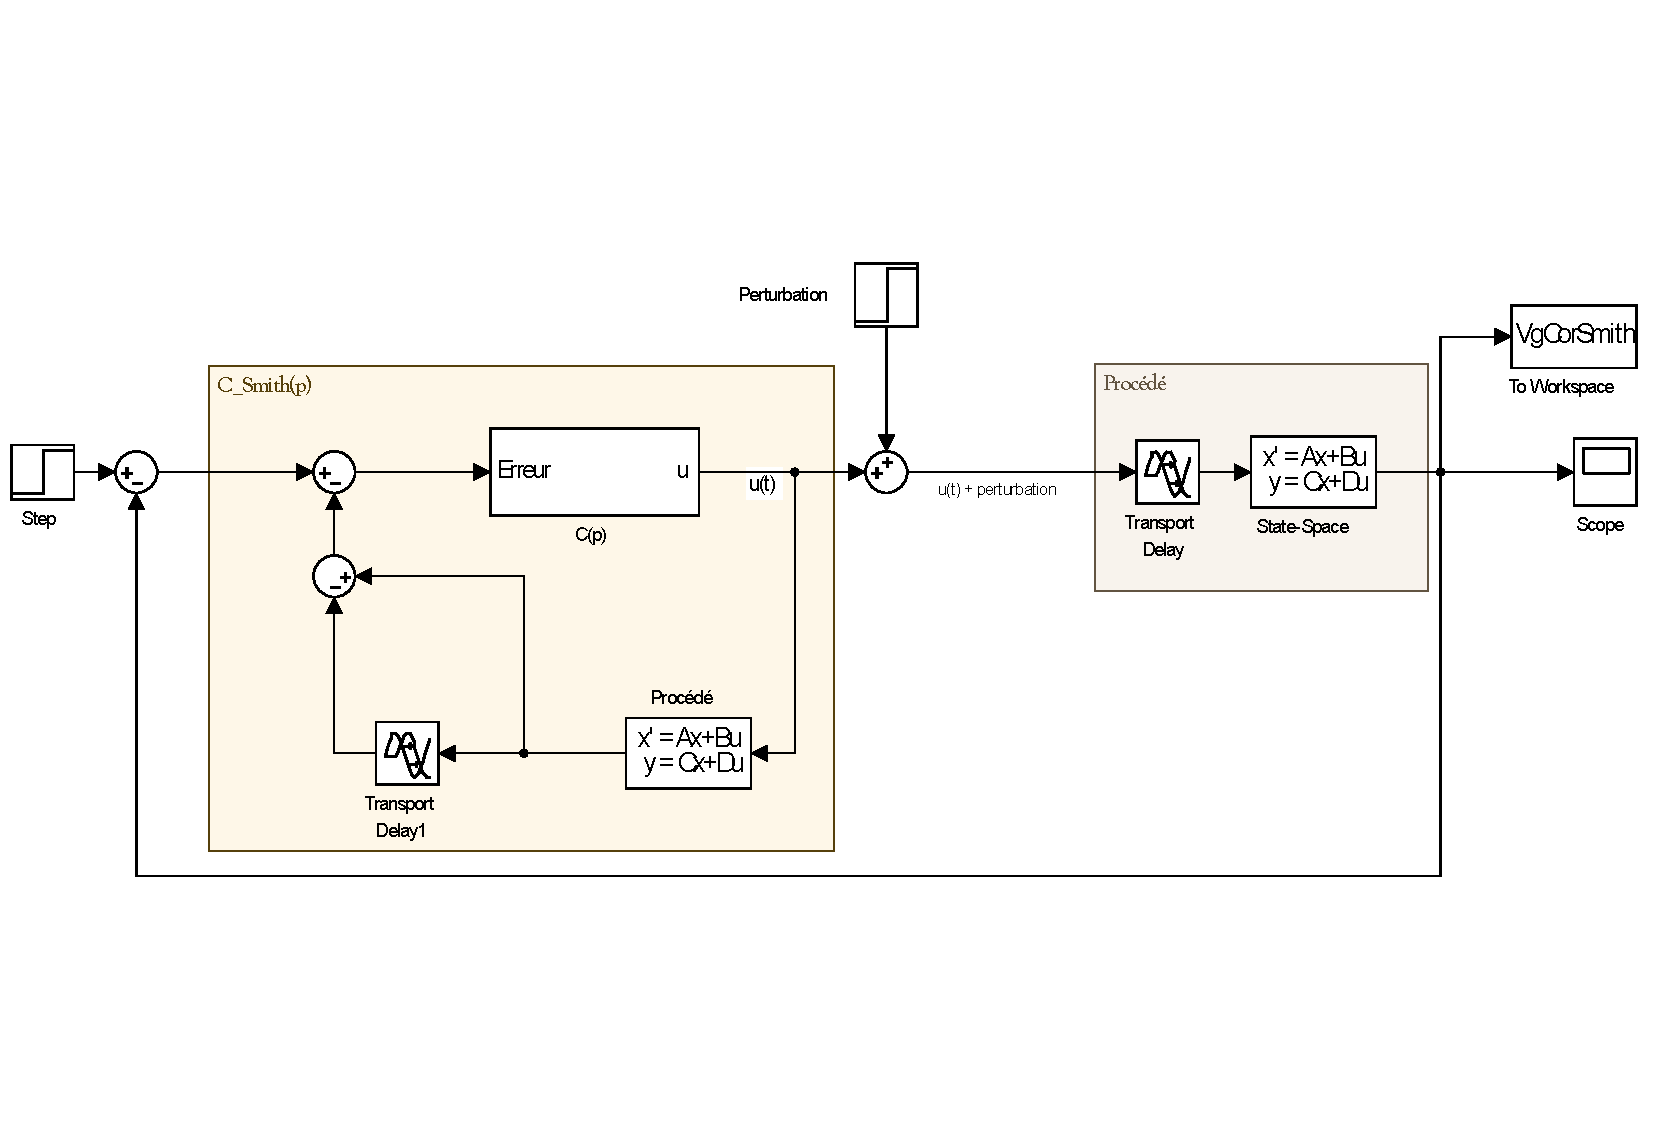
\includegraphics[width=\textwidth]{./IV/images/schema_Predicteur.pdf}
\caption{Schéma de principe du prédicteur de Smith}\label{fig:sch_predicteurSmith}
\end{figure}
Le bloc $C(p)$ devra contenir le bloc de commande que nous souhaitons utiliser. Il pourra être complexe ou bien plus simple.

\section{Fonction de transfert du système en boucle fermé}